\chapter{Evaluation}

\section{Introduzione}
In questo capitolo, sono esaminati i risultati ottenuti dalla \textbf{validazione incrociata} (\textbf{K-fold cross-validation}) sui modelli di classificazione \textbf{Naive Bayes} e \textbf{Support Vector Machine} (\textbf{SVM}). L'obiettivo principale è valutare le prestazioni di ciascun modello in modo sistematico e approfondito, utilizzando un approccio rigoroso basato su \textbf{metriche quantitative}.

Per ottenere un'analisi dettagliata, sono state misurate le performance di entrambi i modelli attraverso metriche chiave come \textbf{accuratezza}, \textbf{matrice di confusione}, \textbf{precisione}, \textbf{recall}, \textbf{F1-score} e \textbf{overfitting}. La \textbf{validazione incrociata} consente di ridurre la variabilità nei risultati e garantire che le \textbf{prestazioni osservate} non dipendano da una particolare suddivisione dei dati. In questo contesto, il \textbf{confronto} tra Naive Bayes e SVM permette di evidenziare differenze significative in termini di \textbf{capacità predittiva}, \textbf{robustezza} e \textbf{adattabilità} a differenti \textbf{distribuzioni dei dati}.

Infine, sono discussi dei possibili \textbf{scenari applicativi} in cui ciascun modello potrebbe risultare più adatto, considerando fattori come la \textbf{sensibilità ai dati sbilanciati}, le \textbf{risorse computazionali richieste} e l'\textbf{interpretabilità del modello}.



\section{Metriche di Valutazione dei Modelli}
Per valutare le prestazioni dei modelli, sono state utilizzate le seguenti metriche:

\begin{itemize}
    \item \textbf{Accuratezza}: misura la percentuale di previsioni corrette rispetto al numero totale di previsioni.
    \begin{equation} Accuracy = \frac{TP+TN}{TP+TN+FP+FN}\end{equation}

    \item \textbf{Precisione} (o \textbf{Positive Predictive Value}): indica la percentuale di previsioni positive corrette rispetto a tutte le previsioni positive fatte dal modello.
    \begin{equation} Precision = \frac{TP}{TP+FP}\end{equation}

    \item \textbf{Recall} (o \textbf{Sensibilità} o \textbf{True Positive Rate}): misura la percentuale di veri positivi identificati correttamente dal modello.
    \begin{equation} Recall = \frac{TP}{TP+FN}\end{equation}

    \item \textbf{F1-score}: è la media armonica di precisione e recall, che bilancia entrambi i valori. È utile quando c'è uno squilibrio tra le classi.\begin{equation} F1 = 2* \frac{Precision*Recall}{Precision+Recall}\end{equation}

    \item \textbf{Overfitting}: misura la differenza tra l'accuratezza sui dati di addestramento e l'accuratezza sui dati di test per valutare la capacit\`a di generalizzazione del modello. Un valore elevato di questa differenza indica che il modello si adatta troppo ai dati di training e potrebbe non generalizzare bene su dati non visti.\begin{equation}Overfitting = Accuracy_{train} - Accuracy_{test}\end{equation}
\end{itemize}

Dove:
\begin{itemize}
    \item \textbf{TP} è il numero di veri positivi,
    \item \textbf{TN} è il numero di veri negativi,
    \item \textbf{FP} è il numero di falsi positivi,
    \item \textbf{FN} è il numero di falsi negativi.
\end{itemize}

\newpage

\section{Risultati del Modello Naive Bayes}

\subsection{Risultati di Addestramento}

Il modello \textbf{Naive Bayes} ha ottenuto un'accuratezza complessiva del \textbf{92.43\%} sui dati di addestramento. Questa performance suggerisce una buona capacità del modello di generalizzare il comportamento delle classi, mantenendo un buon livello di prestazioni anche su dati non visti. \\ \\
La matrice di confusione, che riporta il numero di previsioni corrette e errate per ciascuna classe, mostra i seguenti risultati:

\begin{figure}[H]
    \centering
    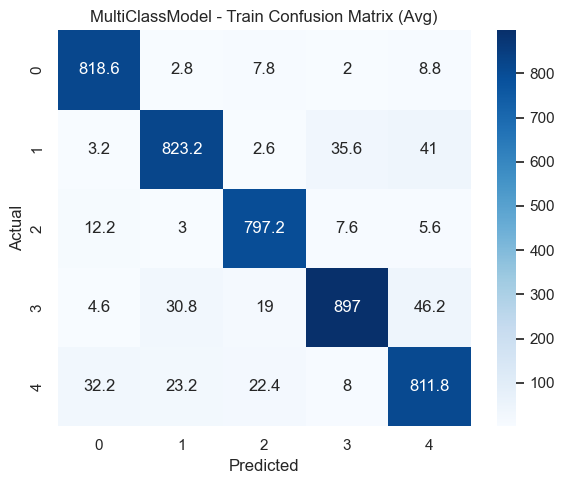
\includegraphics[width=0.8\textwidth]{images/confusion_matrix_train_naive_bayes.png}
    \caption{Matrice di confusione per il training di Naive Bayes}
    \label{fig:confusion_matrix_train_naive_bayes}
\end{figure}

Il modello mostra buone prestazioni complessive, con un'alta percentuale di istanze correttamente classificate, come evidenziato dai valori elevati sulla \textbf{diagonale principale}. Tuttavia, ci sono errori significativi tra alcune classi, in particolare tra le classi 0, 1 e 4, dove il modello ha difficoltà a distinguere correttamente. Per esempio, molte istanze della classe 0 sono state erroneamente classificate come classe 4, e molte istanze della classe 1 sono state scambiate con le classi 3 e 4. Questo evidenzia alcune aree in cui il modello potrebbe migliorare nel riconoscere meglio le differenze tra queste classi.


\newpage

Le metriche per ogni categoria sono mostrate nella seguente tabella e visualizzate nel seguente grafico:

\begin{table}[H]
    \centering
    \begin{tabular}{|c|c|c|c|c|}
        \hline
        \textbf{Categoria} & \textbf{Precision} & \textbf{Recall} & \textbf{F1-score} \\
        \hline
        Accesso & 93.61\% & 96.13\% & 94.85\% \\
        \hline
        Didattica & 93.34\% & 90.82\% & 92.06\% \\
        \hline
        Profilo & 93.55\% & 95.89\% & 94.70\% \\
        \hline
        Segreteria & 94.24\% & 89.51\% & 91.82\% \\
        \hline
        Tecnico & 87.65\% & 90.67\% & 89.14\% \\
        \hline
        Media & 92.48\% & 92.61\% & 92.51\% \\
        \hline
        Media pesata & 92.49\% & 92.44\% & 92.43\% \\
        \hline
    \end{tabular}
    \caption{Confronto tra precision, recall e F1-score per il training di Naive Bayes}
    \label{tab:metriche_naive_bayes_train}
\end{table}

\begin{figure}[H]
    \centering
    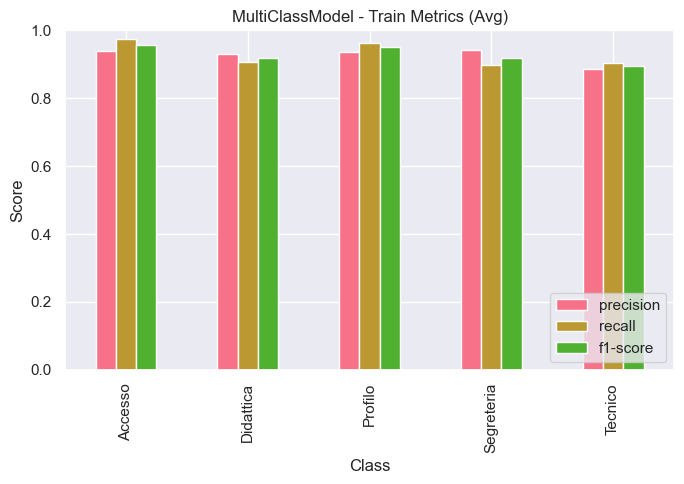
\includegraphics[width=0.8\textwidth]{images/metrics_train_naive_bayes.png}
    \caption{Confronto tra precision, recall e F1-score per il training di Naive Bayes}
    \label{fig:metrics_train_naive_bayes}
\end{figure}

Il modello mostra buone performance complessive, ma nelle categorie \textbf{Segreteria} e \textbf{Tecnico} ci sono margini di miglioramento. \textbf{Segreteria} ha una buona precisione (94.24\%), ma un recall relativamente basso (89.51\%), mentre \textbf{Tecnico} ha un buon recall (90.67\%), ma una precisione più bassa (87.65\%).


\newpage

\subsection{Risultati di Test}

Per quanto riguarda i \textbf{dati di test}, il modello ha ottenuto un'accuratezza del \textbf{88.92\%}, una leggera riduzione rispetto ai dati di addestramento, ma comunque una performance robusta. \\ \\
La matrice di confusione sui dati di test è la seguente:

\begin{figure}[H]
    \centering
    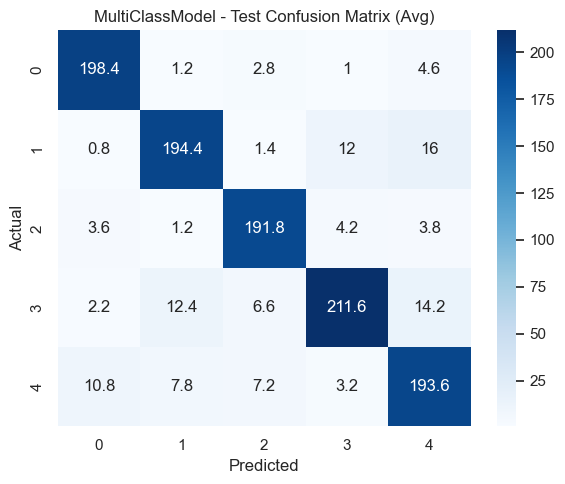
\includegraphics[width=0.8\textwidth]{images/confusion_matrix_test_naive_bayes.png}
    \caption{Matrice di confusione per il testing di Naive Bayes}
    \label{fig:confusion_matrix_test_naive_bayes}
\end{figure}

Mentre le metriche per ogni categoria sono mostrate nella seguente tabella e visualizzate nel seguente grafico:

\begin{table}[H]
    \centering
    \begin{tabular}{|c|c|c|c|c|}
        \hline
        \textbf{Categoria} & \textbf{Precision} & \textbf{Recall} & \textbf{F1-score} \\
        \hline
        Accesso & 90.83\% & 93.38\% & 92.07\% \\
        \hline
        Didattica & 89.35\% & 86.27\% & 87.77\% \\
        \hline
        Profilo & 91.02\% & 93.70\% & 92.33\% \\
        \hline
        Segreteria & 91.67\% & 85.15\% & 88.28\% \\
        \hline
        Tecnico & 82.18\% & 87.25\% & 84.63\% \\
        \hline
        Media & 89.01\% & 89.15\% & 89.02\% \\
        \hline
        Media pesata & 89.05\% & 88.92\% & 88.92\% \\
        \hline
    \end{tabular}
    \caption{Confronto tra precision, recall e F1-score per il testing di Naive Bayes}
    \label{tab:metriche_naive_bayes_test}
\end{table}

\begin{figure}[H]
    \centering
    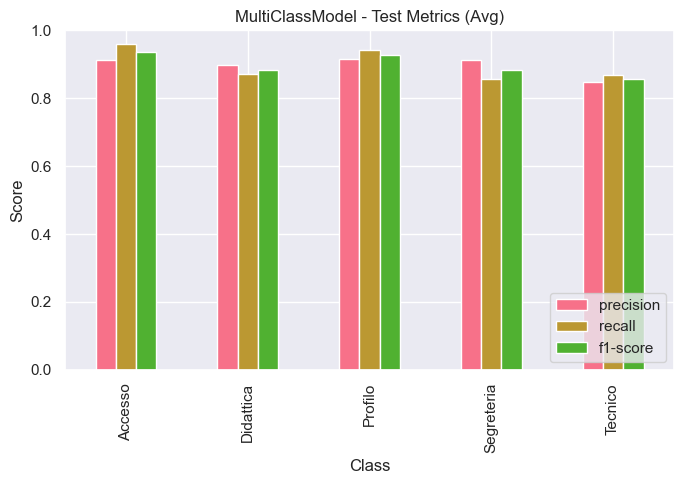
\includegraphics[width=0.8\textwidth]{images/metrics_test_naive_bayes.png}
    \caption{Confronto tra precision, recall e F1-score per il testing di Naive Bayes}
    \label{fig:metrics_test_naive_bayes}
\end{figure}

\subsection{Overfitting}

Per valutare il rischio di \textbf{overfitting}, sono stati analizzati i valori di accuratezza nei diversi fold della validazione incrociata a k-fold. Le differenze tra l'accuratezza dei dati variano tra \textbf{0.02} e \textbf{0.05}, con una media di \textbf{0.0351}. Sebbene vi sia una leggera tendenza all'overfitting, i valori rientrano in un intervallo accettabile, confermando la buona generalizzazione del modello.

\begin{figure}[H]
    \centering
    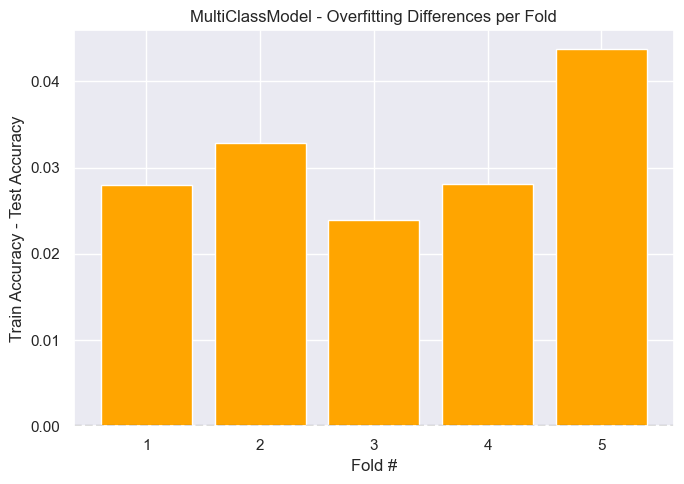
\includegraphics[width=0.8\textwidth]{images/overfitting_naive_bayes.png}
    \caption{Confronto dell'overfitting nei 5 fold per Naive Bayes}
    \label{fig:overfitting_naive_bayes}
\end{figure}

\newpage

\section{Risultati del Modello Support Vector Machine (SVM)}

\subsection{Risultati di Addestramento}

Il modello \textbf{Support Vector Machine (SVM)} ha ottenuto un'accuratezza complessiva del \textbf{92.06\%} sui dati di addestramento. Questo risultato suggerisce una forte capacità del modello nel generalizzare il comportamento delle classi, mantenendo alte prestazioni anche su dati non visti. \\ \\
La matrice di confusione, che riporta il numero di previsioni corrette ed errate per ciascuna classe, è la seguente:

\begin{figure}[H]
    \centering
    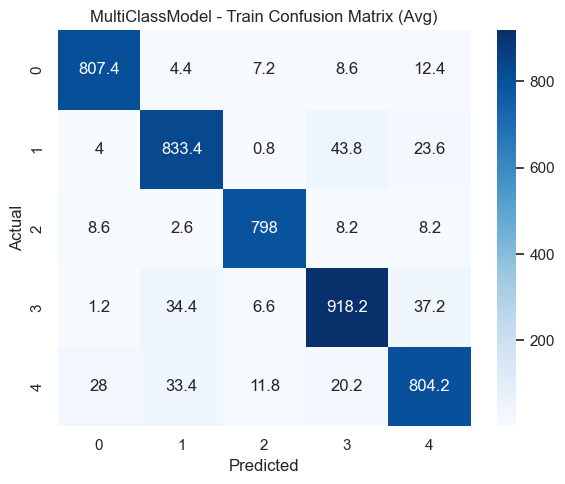
\includegraphics[width=0.8\textwidth]{images/confusion_matrix_train_svm.png}
    \caption{Matrice di confusione per i dati di addestramento con SVM}
    \label{fig:confusion_matrix_train_svm}
\end{figure}

Il modello mostra buone prestazioni complessive, con un'alta percentuale di istanze correttamente classificate, come evidenziato dai valori elevati sulla \textbf{diagonale principale}. Tuttavia, ci sono errori significativi tra alcune classi, in particolare tra le classi 0, 3 e 4, dove il modello ha difficoltà a distinguere correttamente. Per esempio, molte istanze della classe 0 sono state erroneamente classificate come classe 4, mentre la classe 3 ha causato scambi con le classi 1 e 4. Inoltre, la classe 1 ha mostrato confusione con la classe 3, con molte istanze della classe 1 erroneamente classificate come classe 3. Questo evidenzia alcune aree in cui il modello potrebbe migliorare nel riconoscere meglio le differenze tra queste classi .

\newpage

Le metriche per ogni categoria sono mostrate nella seguente tabella e visualizzate nel seguente grafico:

\begin{table}[H]
    \centering
    \begin{tabular}{|c|c|c|c|c|}
        \hline
        \textbf{Categoria} & \textbf{Precision} & \textbf{Recall} & \textbf{F1-score} \\
        \hline
        Accesso & 92.97\% & 93.39\% & 93.18\% \\
        \hline
        Didattica & 91.13\% & 91.80\% & 91.46\% \\
        \hline
        Profilo & 96.49\% & 95.94\% & 96.21\% \\
        \hline
        Segreteria & 91.61\% & 91.21\% & 91.41\% \\
        \hline
        Tecnico & 88.66\% & 88.48\% & 88.57\% \\
        \hline
        Media & 92.17\% & 92.17\% & 92.16\% \\
        \hline
        Media pesata & 92.07\% & 92.07\% & 92.07\% \\
        \hline
    \end{tabular}
    \caption{Confronto tra precision, recall e F1-score per il training di SVM}
    \label{tab:metriche_svm_train}
\end{table}

\begin{figure}[H]
    \centering
    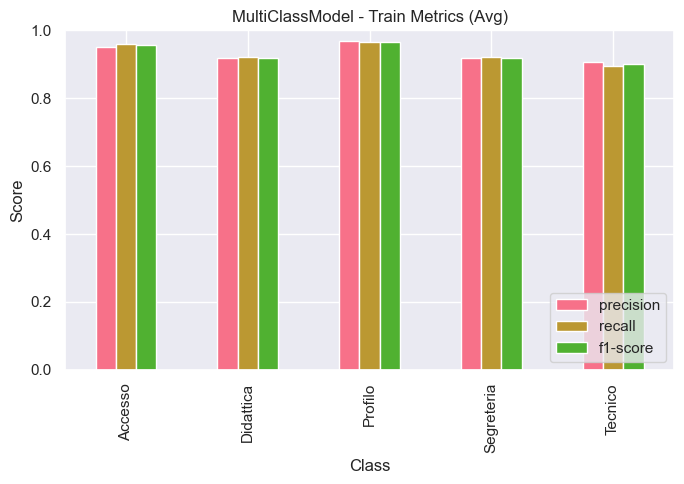
\includegraphics[width=0.8\textwidth]{images/metrics_train_svm.png}
    \caption{Confronto tra precision, recall e F1-score per il training di SVM}
    \label{fig:metrics_train_svm}
\end{figure}

Il modello mostra buone performance complessive, ma nelle categorie \textbf{Tecnico} e \textbf{Didattica} ci sono margini di miglioramento. \textbf{Tecnico} ha una buona precisione (88.66\%), ma un recall relativamente basso (88.48\%), mentre \textbf{Didattica} ha un buon recall (91.80\%), ma una precisione più bassa (91.13\%).

\newpage

\subsection{Risultati di Test}

Per quanto riguarda i \textbf{dati di test}, il modello ha ottenuto un'accuratezza del \textbf{89.95\%}, con una leggera riduzione rispetto ai dati di addestramento, ma comunque una performance robusta. \\ \\
La matrice di confusione sui dati di test è la seguente:

\begin{figure}[H]
    \centering
    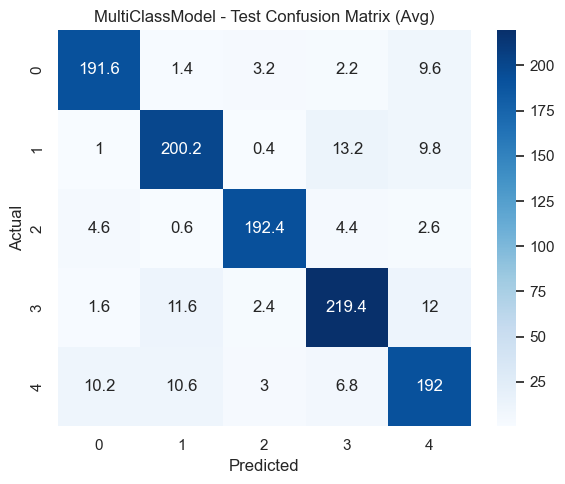
\includegraphics[width=0.8\textwidth]{images/confusion_matrix_test_svm.png}
    \caption{Matrice di confusione per i dati di test con SVM}
    \label{fig:confusion_matrix_test_svm}
\end{figure}

Mentre le metriche per ogni categoria sono mostrate nella seguente tabella e visualizzate nel seguente grafico:

\begin{table}[H]
    \centering
    \begin{tabular}{|c|c|c|c|c|}
        \hline
        \textbf{Categoria} & \textbf{Precision} & \textbf{Recall} & \textbf{F1-score} \\
        \hline
        Accesso & 91.67\% & 92.14\% & 91.89\% \\
        \hline
        Didattica & 89.19\% & 89.07\% & 89.13\% \\
        \hline
        Profilo & 95.50\% & 94.02\% & 94.74\% \\
        \hline
        Segreteria & 89.14\% & 88.81\% & 88.97\% \\
        \hline
        Tecnico & 85.14\% & 86.27\% & 85.69\% \\
        \hline
        Media & 90.13\% & 90.06\% & 90.08\% \\
        \hline
        Media pesata & 90.01\% & 89.95\% & 89.97\% \\
        \hline
    \end{tabular}
    \caption{Confronto tra precision, recall e F1-score per il testing di SVM}
    \label{tab:metriche_svm_test}
\end{table}

\begin{figure}[H]
    \centering
    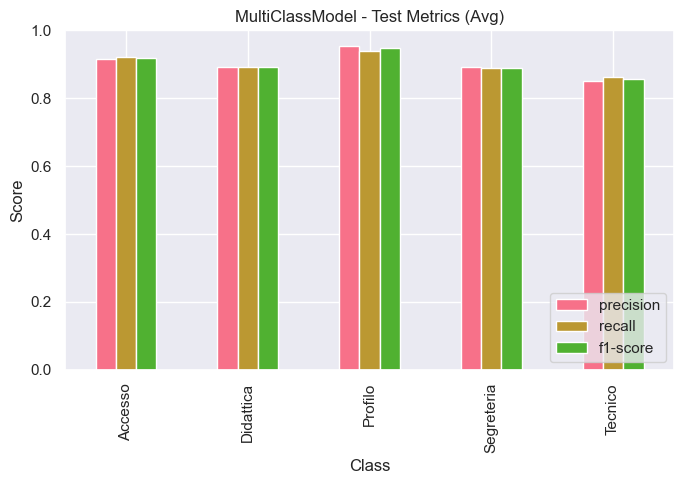
\includegraphics[width=0.8\textwidth]{images/metrics_test_svm.png}
    \caption{Confronto tra precision, recall e F1-score per il testing di SVM}
    \label{fig:metrics_test_svm}
\end{figure}

\subsection{Overfitting}

Per valutare il rischio di \textbf{overfitting}, sono stati analizzati i valori di accuratezza nei diversi fold della validazione incrociata a k-fold. Le differenze tra l'accuratezza dei dati variano tra \textbf{0.01} e \textbf{0.04}, con una media di \textbf{0.0211}. Sebbene vi sia una leggera tendenza all'overfitting, i valori rientrano in un intervallo accettabile, confermando la buona generalizzazione del modello.

\begin{figure}[H]
    \centering
    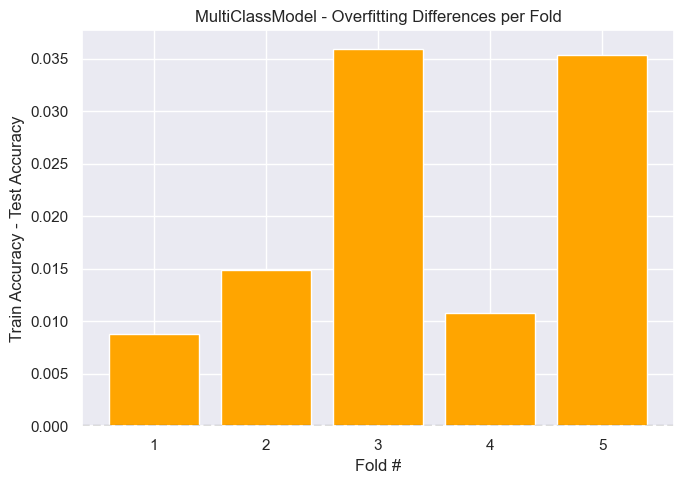
\includegraphics[width=0.8\textwidth]{images/overfitting_svm.png}
    \caption{Confronto dell'overfitting nei 5 fold per SVM}
    \label{fig:overfitting_svm}
\end{figure}

\newpage

\section{Confronto tra i Modelli}

\subsection{Prestazioni Complessive}

Entrambi i modelli, \textbf{Naive Bayes} e \textbf{SVM}, mostrano prestazioni molto simili. Durante il training, \textbf{Naive Bayes} raggiunge un'accuratezza del 92.44\%, mentre \textbf{SVM} è leggermente migliore con un'accuratezza del 92.07\%. Quando testati sui dati di test, entrambi i modelli registrano una piccola diminuzione delle performance, con \textbf{Naive Bayes} che scende al 88.92\% e \textbf{SVM} che ottiene il 89.95\%. Le metriche di precisione, recall e f1-score sono anch'esse molto simili per entrambi i modelli, suggerendo che entrambi sono abbastanza equilibrati nel bilanciare la capacità di classificare correttamente le istanze e nel ridurre al minimo gli errori.

\begin{table}[H]
    \centering
    \begin{tabular}{|c|c|c|c|c|c|}
        \hline
        \textbf{Modello} & \textbf{Set} & \textbf{Accuracy} & \textbf{Precision} & \textbf{Recall} & \textbf{F1-score} \\
        \hline
        Naive Bayes & Training & 92.44\% & 92.49\% & 92.44\% & 92.43\% \\
        \hline
        Naive Bayes & Test & 88.92\% & 89.05\% & 88.92\% & 88.92\% \\
        \hline
        SVM & Training & 92.07\% & 92.17\% & 92.07\% & 92.07\% \\
        \hline
        SVM & Test & 89.95\% & 90.01\% & 89.95\% & 89.97\% \\
        \hline
    \end{tabular}
    \caption{Confronto tra i modelli in termini di accuracy, precision, recall e F1-score}
    \label{tab:confronto_metriche}
\end{table}


\subsection{Overfitting}

Sia il modello \textbf{Naive Bayes} che il modello \textbf{SVM} mostrano una lieve presenza di \textbf{overfitting}, con differenze tra le performance sui dati che variano tra \textbf{0.01} e \textbf{0.05} per Naive Bayes e tra \textbf{0.01} e \textbf{0.04} per SVM. Le differenze medie sono però significative: Naive Bayes ha una differenza media di \textbf{0.0351}, mentre SVM di \textbf{0.0211}, suggerendo che SVM ha una prestazione più stabile. L'andamento dell'overfitting è stato visualizzato calcolando le differenze per ogni fold del \textbf{k-fold cross-validation}, come mostrato nell'immagine seguente, che confronta i due modelli.

\begin{figure}[H]
    \centering
    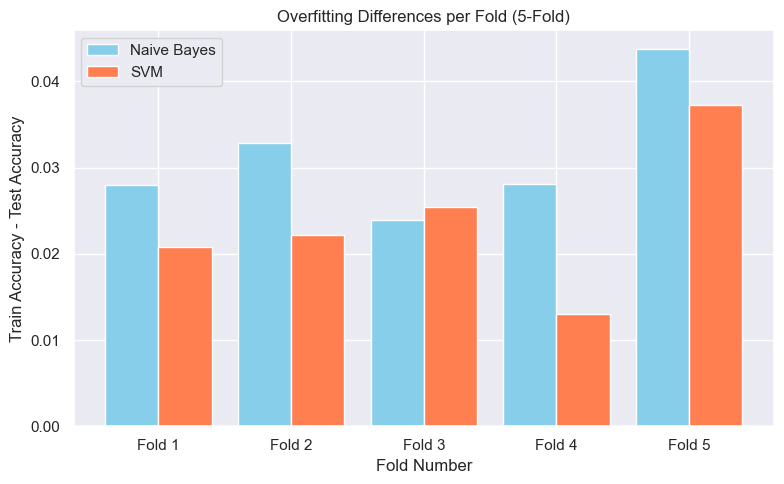
\includegraphics[width=0.8\textwidth]{images/overfitting_differences.png}
    \caption{Confronto dell'overfitting tra Naive Bayes e SVM}
    \label{fig:overfitting_differences}
\end{figure}

\section{Conclusioni}

Entrambi i modelli, Naive Bayes e Support Vector Machine (SVM), hanno mostrato prestazioni eccellenti nel compito di \textbf{classificazione}, evidenziando differenze minime nelle metriche di valutazione. Sebbene il modello SVM ottenga risultati leggermente migliori in termini di accuratezza sui dati di test, con un’accuratezza del \textbf{89.95\%} rispetto al \textbf{88.92\%} di Naive Bayes, la differenza tra i due modelli è contenuta. Inoltre, i dati sull'overfitting suggeriscono che SVM presenta una prestazione più stabile, con una minore differenza media tra i fold della \textbf{validazione incrociata}, rispetto a Naive Bayes. Questo indica che entrambi i modelli sono ben calibrati per il compito e sono capaci di generalizzare efficacemente.

\textbf{Naive Bayes}, grazie alla sua semplicità e velocità di esecuzione, potrebbe essere la scelta preferibile in scenari con risorse computazionali limitate o in situazioni che richiedono modelli facilmente interpretabili. La sua capacità di gestire grandi volumi di dati con risorse relativamente basse lo rende adatto per applicazioni in tempo reale o su dispositivi con risorse limitate.

D’altra parte, \textbf{SVM} si distingue per una maggiore precisione in alcuni casi, ed è generalmente considerato una scelta solida quando è necessaria maggiore accuratezza e quando sono disponibili risorse computazionali adeguate. Inoltre, SVM è più adatto per situazioni che richiedono una maggiore capacità di generalizzazione.

In definitiva, entrambi i modelli sono validi per il problema in esame e presentano un buon compromesso tra \textbf{accuratezza} e capacità di \textbf{generalizzazione}. La scelta finale tra Naive Bayes e SVM dipenderà da considerazioni specifiche, come la disponibilità di risorse computazionali, la necessità di interpretabilità del modello e la priorità data a una leggera miglioria nelle prestazioni rispetto alla velocità di esecuzione. 